\documentclass[11pt]{article}

\usepackage{fullpage} % Package to use full page
\usepackage{parskip} % Package to tweak paragraph skipping
\usepackage{tikz} % Package for drawing
\usepackage{amsmath}
\usepackage{hyperref}
\usepackage{graphicx}
\usepackage{authblk}
\usepackage{natbib}
\usepackage{multirow}

%%%%%%%%%%%%%%%%%%%%%%%%%%%%%%%%%
\setlength{\textheight}{9in}
\setlength{\topmargin}{-0.600in}
\setlength{\headheight}{0.2in}
\setlength{\headsep}{0.250in}
\setlength{\footskip}{0.5in}
\flushbottom
\setlength{\textwidth}{6.5in}
\setlength{\oddsidemargin}{0in}
\setlength{\evensidemargin}{0in}
\setlength{\columnsep}{2pc}
\setlength{\parindent}{1em}
%%%%%%%%%%%%%%%%%%%%%%%%%%%%%%%%%

\title{AlphaEpsilon: An implementation of AlphaZero within some $\varepsilon$ neighborhood.}
\author{Travis Tiner}
\author{Josh Tracy}
\author{Kali Wickens}
\affil{University of Utah -- Deep Learning}
\date{\today}

\begin{document}

\maketitle

\section{Introduction}

	%! Author = kaliw
%! Date = 12/9/2019

% Introduction





\section{TicTacToe}

	%! Author = kaliw
%! Date = 12/10/2019

% TicTacToe Game


\section{The Players}

	%! Author = kaliw
%! Date = 12/10/2019

% Random Player
\subsection{The Random Agent (aka Charmander)}
In order to begin our training set, we built our random agent, which we will call Charmander.
Much to be expected, this quaint little model wasn't very powerful.
In a 1000 games, while playing itself, the X player only won about 60\% of the time.
The X player always has the advantage due to having the first move, thus these results were not promising, though expected.

	%! Author = kaliw
%! Date = 12/10/2019

% Dense Net
\subsection{The Dense Player (aka Charmeleon)}

Our first neural net we developed, Charmeleon, was created using a deep, fully connected  network.
The network architecture we use is:
\begin{enumerate}
	\item Fully Connected 400x1
	\item ReLU
	\item Dropout (0.2)
	\item Fully Connected 300x1
	\item ReLU
	\item Fully Connected 200x1
	\item ReLU
	\item Fully Connected 125
	\item ReLU
	\item Fully Connected 75
	\item ReLU
	\item Dropout (0.1)
	\item Fully Connected 25x1
	\item ReLU
	\item Fully Connected 3x1
	\item Softmax
\end{enumerate}
This model takes a flattened game board as input as x, and the array [win, loss, draw] as y. It then evaluates the board states, learning whether a specific board state corresponding to either a win, loss, or draw. A few rounds of trial and error landed us on this specific architecture. Against the random model, it performed quite well, raising the win percentage from 60\% to 88\%. The full results of the modoels can be seen below in Table 1. 

For this model, we used an Adam optimizer with a learning rate of 0.0001, $\beta_1$ of 0.9 and $\beta_2$ of 0.999. Below you can see how results of the training runs:

\begin{figure}[h!]
	\centering
	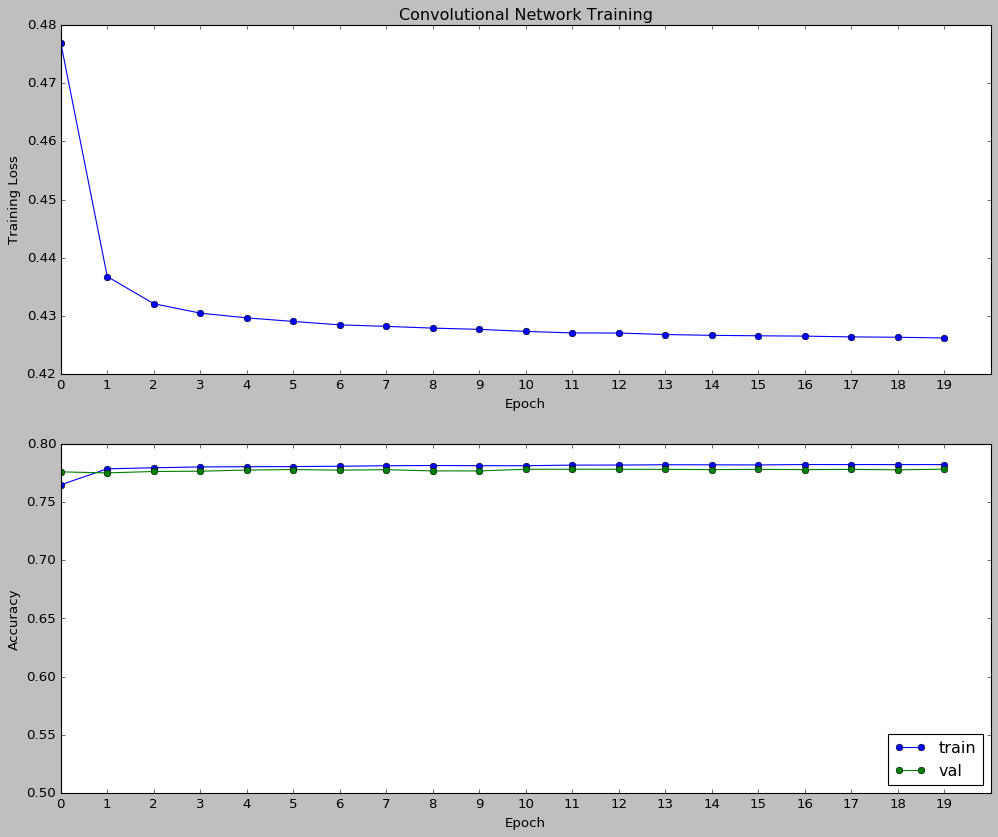
\includegraphics[width=10cm, height=7cm]{convolutional-net-training.png}
	\caption{Top: Training loss over 20 epochs. Bottom: Training accuracy against validation accuracy over 20 epochs}
	\label{fig:conv_net}
\end{figure}

	%! Author = kaliw
%! Date = 12/10/2019

% Convolutional Net
\subsection{The Convolutional Player (aka Charizard)}

Our most evolved net Charizard, was created using a convolutional neural network.
The network architecture we use is:
\begin{enumerate}
    \item Convolution 32@2x2
    \item Batch Normalization
    \item ReLU
    \item Convolution 64@2x2
    \item Batch Normalization
    \item ReLU
    \item Convolution 32@2x2
    \item Fully Connected 512x1
    \item Fully Connected 128x1
    \item Fully Connected 3x1
    \item Softmax
\end{enumerate}
We tried a few different network architectures to see what would work best.  We didn't create a very deep network as tic-tac-toe is a simple game.  The deeper networks that were tried took more time to compute and didn't return far superior results.

We used an Adam optimizer with a learning rate of 0.0001, $\beta_1$ of 0.9 and $\beta_2$ of 0.999. One thing that seemed interesting was that our training and validation accuracy didn't change very much after the first couple epochs. I think part of the issue may be that without Monte Carlo Tree Search, using only random board states we don't see the best board states as frequently as we'd like and thus the network isn't learning as much about the best board states. In a future iteration it would be nice to implement MCTS as well as a temporal dimension.

These are the results of the training runs:
\begin{figure}[h!]
	\centering
	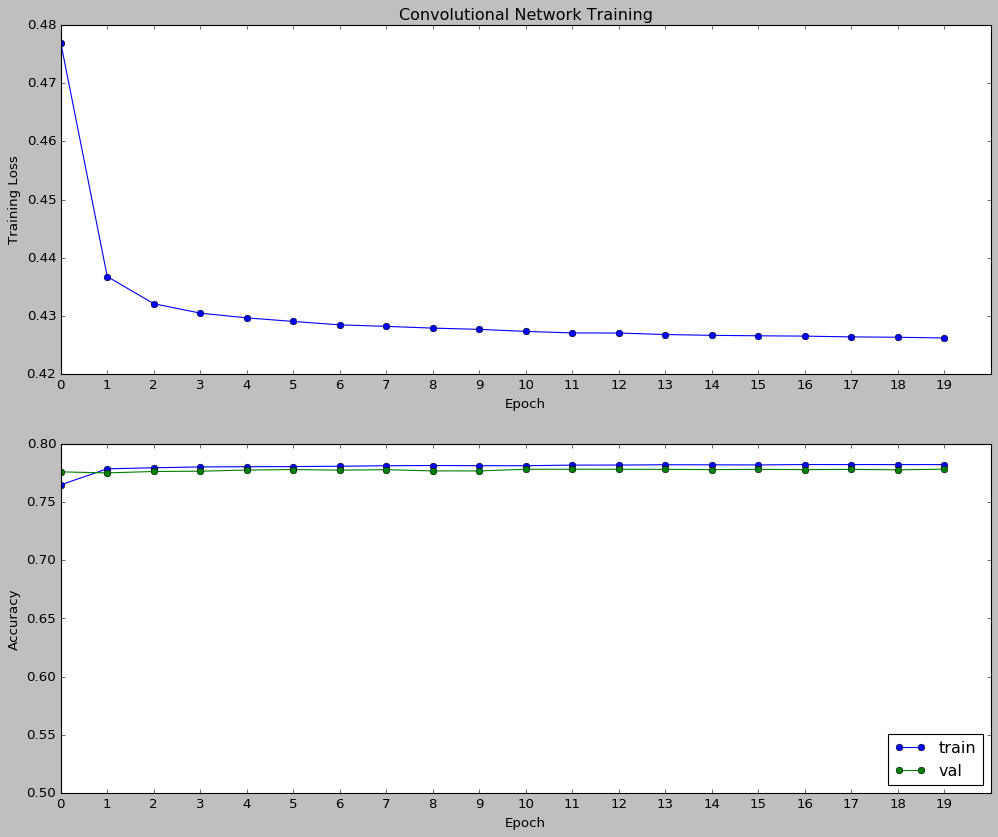
\includegraphics[width=10cm, height=7cm]{convolutional-net-training.png}
	\caption{Top: Training loss over 20 epochs. Bottom: Training accuracy against validation accuracy over 20 epochs}
	\label{fig:conv_net}
\end{figure}


\begin{table}[]
	\centering
	\begin{tabular}{llll}
	\hline
	\textbf{Player} & \textbf{X Wins} & \textbf{O Wins} & \textbf{Draw} \\ \hline
	Random          & 61.1\%          & 27.6\%          & 11.3\%        \\
	Dense           & 63.7\%          & 0.4\%           & 35.9\%        \\
	Convolutional   & 90\%            & 0.4\%           & 9.6\%         \\ \hline
	\end{tabular}
	\caption{Win percentages for each of the players given 1000 games.}
\end{table}

\section{Training and Validation}

	%! Author = kaliw
%! Date = 12/10/2019

% Training and Validation


\section{Human vs Player}

	
	
	


Another way to evaluate the different agents is to play against them.
To do this, we wrote a script called \texttt{human\_v\_model.py} which lets a human agent choose which model agent to play against.
Below we show what each agent's game against a human agent looked like.
For all of the images below, we tried to follow roughly the same move set so that we could see how the bots reacted differently.
The human player went first each time (X) and the agent went second (O:

First up, we will play the random agent, Charmander.
This agent will pick one of the available spaces to play using a random integer generator.
\begin{figure}[H]
	\centering
	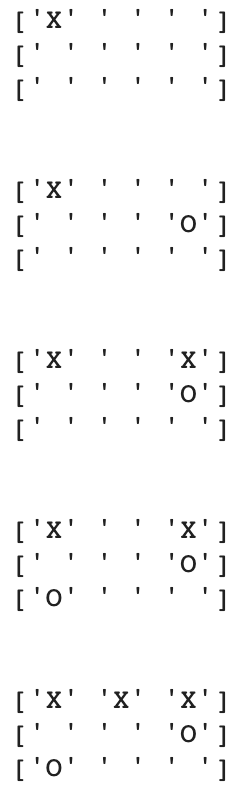
\includegraphics[scale=.5]{h_v_random}
\end{figure}
As you can see, this does not perform well.
Because it's random, it doesn't identify any potential defensive moves or offensive moves.

Next up, we will play our Dense Neural Network agent, Charmeleon.
We expect that this agent will be a stark improvement to the random agent.

\begin{figure}[H]
	\centering
	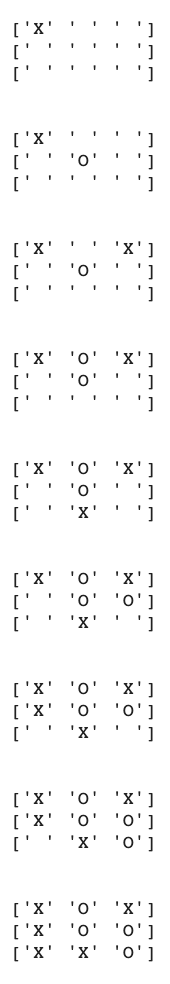
\includegraphics[scale=.5]{h_v_dense}
\end{figure}

First of all, we can see that the dense agent recognizes that it needs to play at row 1, column 2 to block the first attempt for X to win.
It then recognizes that it should play somewhere in row 2 on its next move so that it has a chance to win if X fails to block it.
If it were to play somewhere in row 3 here, it would have no chance to win.
After this move was blocked, though, is where the agent seemed to falter.
For some reason it doesn't identify that X can win in column 1 and fails to block it, resulting in the human agent winning.

Now we will play our Convolutional Neural Network agent, Charizard.
This agent performed marginally better statistically when playing the two other model agents, so we will hopefully see some better performance here.

\begin{figure}[H]
	\centering
	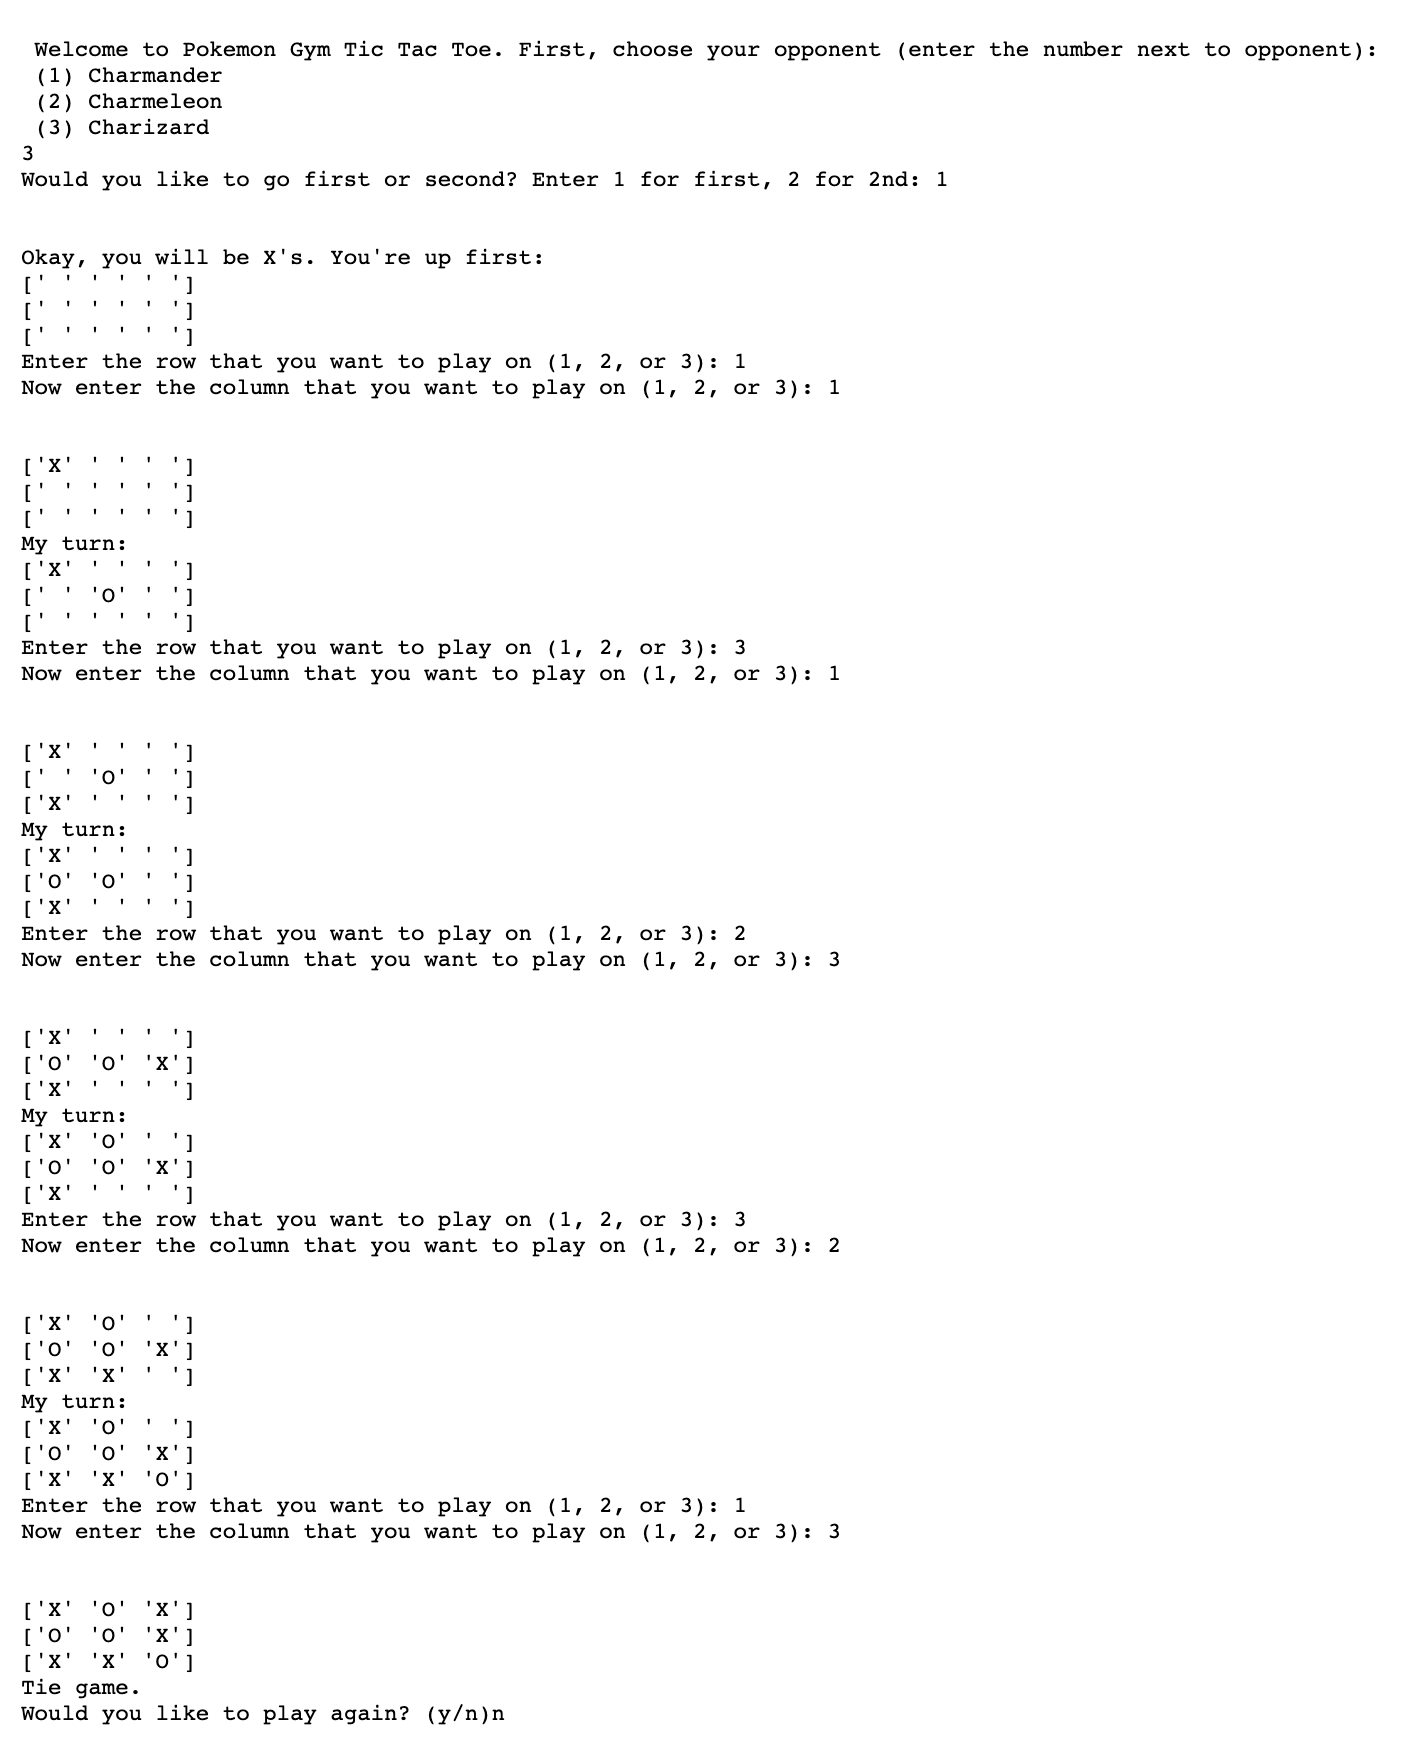
\includegraphics[scale=.5]{h_v_conv}
\end{figure}

Like the dense agent, this convolutional agent identifies and follows its best strategy early in the game.
We can see, however, that this agent correctly identifies the final chance for X to win and blocks it, resulting in a tie game.



	Random change.

%\nocite{*}
%
%\newpage{}
%
%\bibliographystyle{ieeetr}
%
%\bibliography{bibliography}

\end{document}
